\documentclass[]{article}
\usepackage{lmodern}
\usepackage{amssymb,amsmath}
\usepackage{ifxetex,ifluatex}
\usepackage{fixltx2e} % provides \textsubscript
\ifnum 0\ifxetex 1\fi\ifluatex 1\fi=0 % if pdftex
  \usepackage[T1]{fontenc}
  \usepackage[utf8]{inputenc}
\else % if luatex or xelatex
  \ifxetex
    \usepackage{mathspec}
    \usepackage{xltxtra,xunicode}
  \else
    \usepackage{fontspec}
  \fi
  \defaultfontfeatures{Mapping=tex-text,Scale=MatchLowercase}
  \newcommand{\euro}{€}
\fi
% use upquote if available, for straight quotes in verbatim environments
\IfFileExists{upquote.sty}{\usepackage{upquote}}{}
% use microtype if available
\IfFileExists{microtype.sty}{%
\usepackage{microtype}
\UseMicrotypeSet[protrusion]{basicmath} % disable protrusion for tt fonts
}{}
\usepackage[margin=1in]{geometry}
\usepackage{graphicx}
\makeatletter
\def\maxwidth{\ifdim\Gin@nat@width>\linewidth\linewidth\else\Gin@nat@width\fi}
\def\maxheight{\ifdim\Gin@nat@height>\textheight\textheight\else\Gin@nat@height\fi}
\makeatother
% Scale images if necessary, so that they will not overflow the page
% margins by default, and it is still possible to overwrite the defaults
% using explicit options in \includegraphics[width, height, ...]{}
\setkeys{Gin}{width=\maxwidth,height=\maxheight,keepaspectratio}
\ifxetex
  \usepackage[setpagesize=false, % page size defined by xetex
              unicode=false, % unicode breaks when used with xetex
              xetex]{hyperref}
\else
  \usepackage[unicode=true]{hyperref}
\fi
\hypersetup{breaklinks=true,
            bookmarks=true,
            pdfauthor={Eric F. Lock},
            pdftitle={Analysis of gene time course data using MultiwayClassification},
            colorlinks=true,
            citecolor=blue,
            urlcolor=blue,
            linkcolor=magenta,
            pdfborder={0 0 0}}
\urlstyle{same}  % don't use monospace font for urls
\setlength{\parindent}{0pt}
\setlength{\parskip}{6pt plus 2pt minus 1pt}
\setlength{\emergencystretch}{3em}  % prevent overfull lines
\setcounter{secnumdepth}{0}

%%% Use protect on footnotes to avoid problems with footnotes in titles
\let\rmarkdownfootnote\footnote%
\def\footnote{\protect\rmarkdownfootnote}

%%% Change title format to be more compact
\usepackage{titling}

% Create subtitle command for use in maketitle
\newcommand{\subtitle}[1]{
  \posttitle{
    \begin{center}\large#1\end{center}
    }
}

\setlength{\droptitle}{-2em}
  \title{Analysis of gene time course data using MultiwayClassification}
  \pretitle{\vspace{\droptitle}\centering\huge}
  \posttitle{\par}
  \author{Eric F. Lock}
  \preauthor{\centering\large\emph}
  \postauthor{\par}
  \predate{\centering\large\emph}
  \postdate{\par}
  \date{2016-06-26}



\begin{document}

\maketitle


This vignette illustrates the use of the \textbf{MultiwayClassification}
package, using publicly available data on gene time course data
originally described in Baranzini et al. (2005). This package performs
linear classification for data with multi-way structure. The
distance-weighted discrimination (DWD) or support vector machine (SVM)
classification objectives are optimized under the assumption that the
multi-way coefficients have low rank.

\subsection{Loading the data}\label{loading-the-data}

First, if you have not done so already, install and load the package via
GitHub. This package depends on the packages \textbf{DWD} (for DWD) and
\textbf{kernlab} (for SVM). DWD is not currently available on CRAN, and
so will need to be installed via its url:

\begin{verbatim}
install.packages("https://cran.r-project.org/src/contrib/Archive/DWD/DWD_0.11.tar.gz",repos = NULL, type = "source")
library(DWD)
\end{verbatim}

The \textbf{MultiwayClassification} package can then be installed,
directly from GitHub, using the devtools library.

\begin{verbatim}
install.packages(devtools)
library(devtools)
install_github("lockEF/MultiwayClassification")
library(MultiwayClassification)
\end{verbatim}

To load the gene time course data,
enter\\\texttt{data(IFNB\_Data)}\\These data are for patients with
multiple sclerosis after treatment with IFNBeta. Patients are classified
as good or poor responders. Gene expression was measured for 76 genes of
interest before treatment (baseline) and at 6 follow-up time points over
the next two years (3 months, 6 months, 9 months, 12 months, 18 months,
24 months). The original data has been log-normalized and mean-imputed.
The previous command loads the following variables:

\begin{itemize}
\itemsep1pt\parskip0pt\parsep0pt
\item
  \texttt{DataArray}: Time course array: 53 patients X 7 time points X
  76 genes.
\item
  \texttt{Class}: Vector giving patient classification as good or poor
  responders.
\end{itemize}

We will also define the following variables:

\texttt{n\_times=7; n\_genes=76; n\_people=53}

\subsection{DWD classification and
cross-validation}\label{dwd-classification-and-cross-validation}

First, we apply standard DWD on the vectorized data (this corresponds to
the full rank model). Combine the data into a matrix in which each
column gives gene expression for all time points for a given individual:

\begin{verbatim}
FullMat <- matrix(nrow=n_times*n_genes,ncol=n_people)
for(i in 1:n_people){
  FullMat[,i] =  as.vector(DataArray[i,,])
}
\end{verbatim}

Now, use the \texttt{kdwd} function from package \textbf{DWD} to
estimate the separating hyperplane:

\begin{verbatim}
results.full <- kdwd(x=t(FullMat),y=as.factor(Class), scaled=FALSE)
\end{verbatim}

Compute scores for each subject under leave one out cross-validation:

\begin{verbatim}
cv.full = c()
for(i in 1:length(Class)){
  results.full.cv <- kdwd(t(FullMat[,-i]),y=as.factor(Class[-i]), scaled=FALSE)
  cv.full[i] = t(FullMat[,i]) %*%results.full.cv@w[[1]]+results.full.cv@b0[[1]]
}
\end{verbatim}

Now, use the \texttt{mul.dwd} function to estimate the rank 1 multiway
DWD model and compute the scores under leave-one-out cross validation:

\begin{verbatim}
cv.mw = c()
for(i in 1:length(Class)){
  results.mw.cv <-mul.dwd(DataArray[-i,,],y=Class[-i],rank=1)
  cv.mw[i] = sum(DataArray[i,,]*results.mw.cv$beta)+results.mw.cv$int
}
\end{verbatim}

Compare cross validation miss-classification rates for the full and rank
1 model:

\begin{verbatim}
miss.full <- sum(Class==1&cv.full<0 | Class==2&cv.full>0)/length(Class)  #22.6%
miss.mw <- sum(Class==1&(cv.mw+0.1)<0 | Class==2&(cv.mw+0.1)>0)/length(Class) #16.9%
\end{verbatim}

Compare t-statistics under cross-validation between the full rank DWD
and rank 1 model:

\begin{verbatim}
t.test(cv.mw[Class==1],cv.mw[Class==2])$statistic
t.test(cv.full[Class==1],cv.full[Class==2])$statistic 
\end{verbatim}

By setting \texttt{rank=r} in the \texttt{mul.dwd} function, we can
similarly compute the misclassification rate for other rank models.

Finally, we plot the cross-validated scores for each class under the
rank 1 multi-way model, using the package \textbf{ggplot2} for plotting
and \textbf{ks} for kernel density estimates (these packages may need to
be installed beforehand):

\begin{verbatim}
library("ggplot2")
library(ks)
png(filename = "TimeCourseScores_INFB.png",width=8,height=4.5,units='in',res=800)
plot(kde(cv.mw[Class==1],h=1),ylim = c(0,0.22), col='gray', xlim=c(-8,8),xlab = 'Score', ylab = 'Density', lty =2,lwd=2,main = 'Rank 1 multi-way model for MS data')
points(cv.mw[Class==1],runif(20,0.11,0.18),col='black', pch = 'x')
plot(kde(cv.mw[Class==2],h=1), col='gray', add=TRUE, lwd=2)
points(cv.mw[Class==2],runif(33,0.11,0.18),col='black')
legend("topright", legend = c("Good responders", "Bad responders"), pch = c('o', 'x'), lty = c(1, 2))
dev.off()
\end{verbatim}

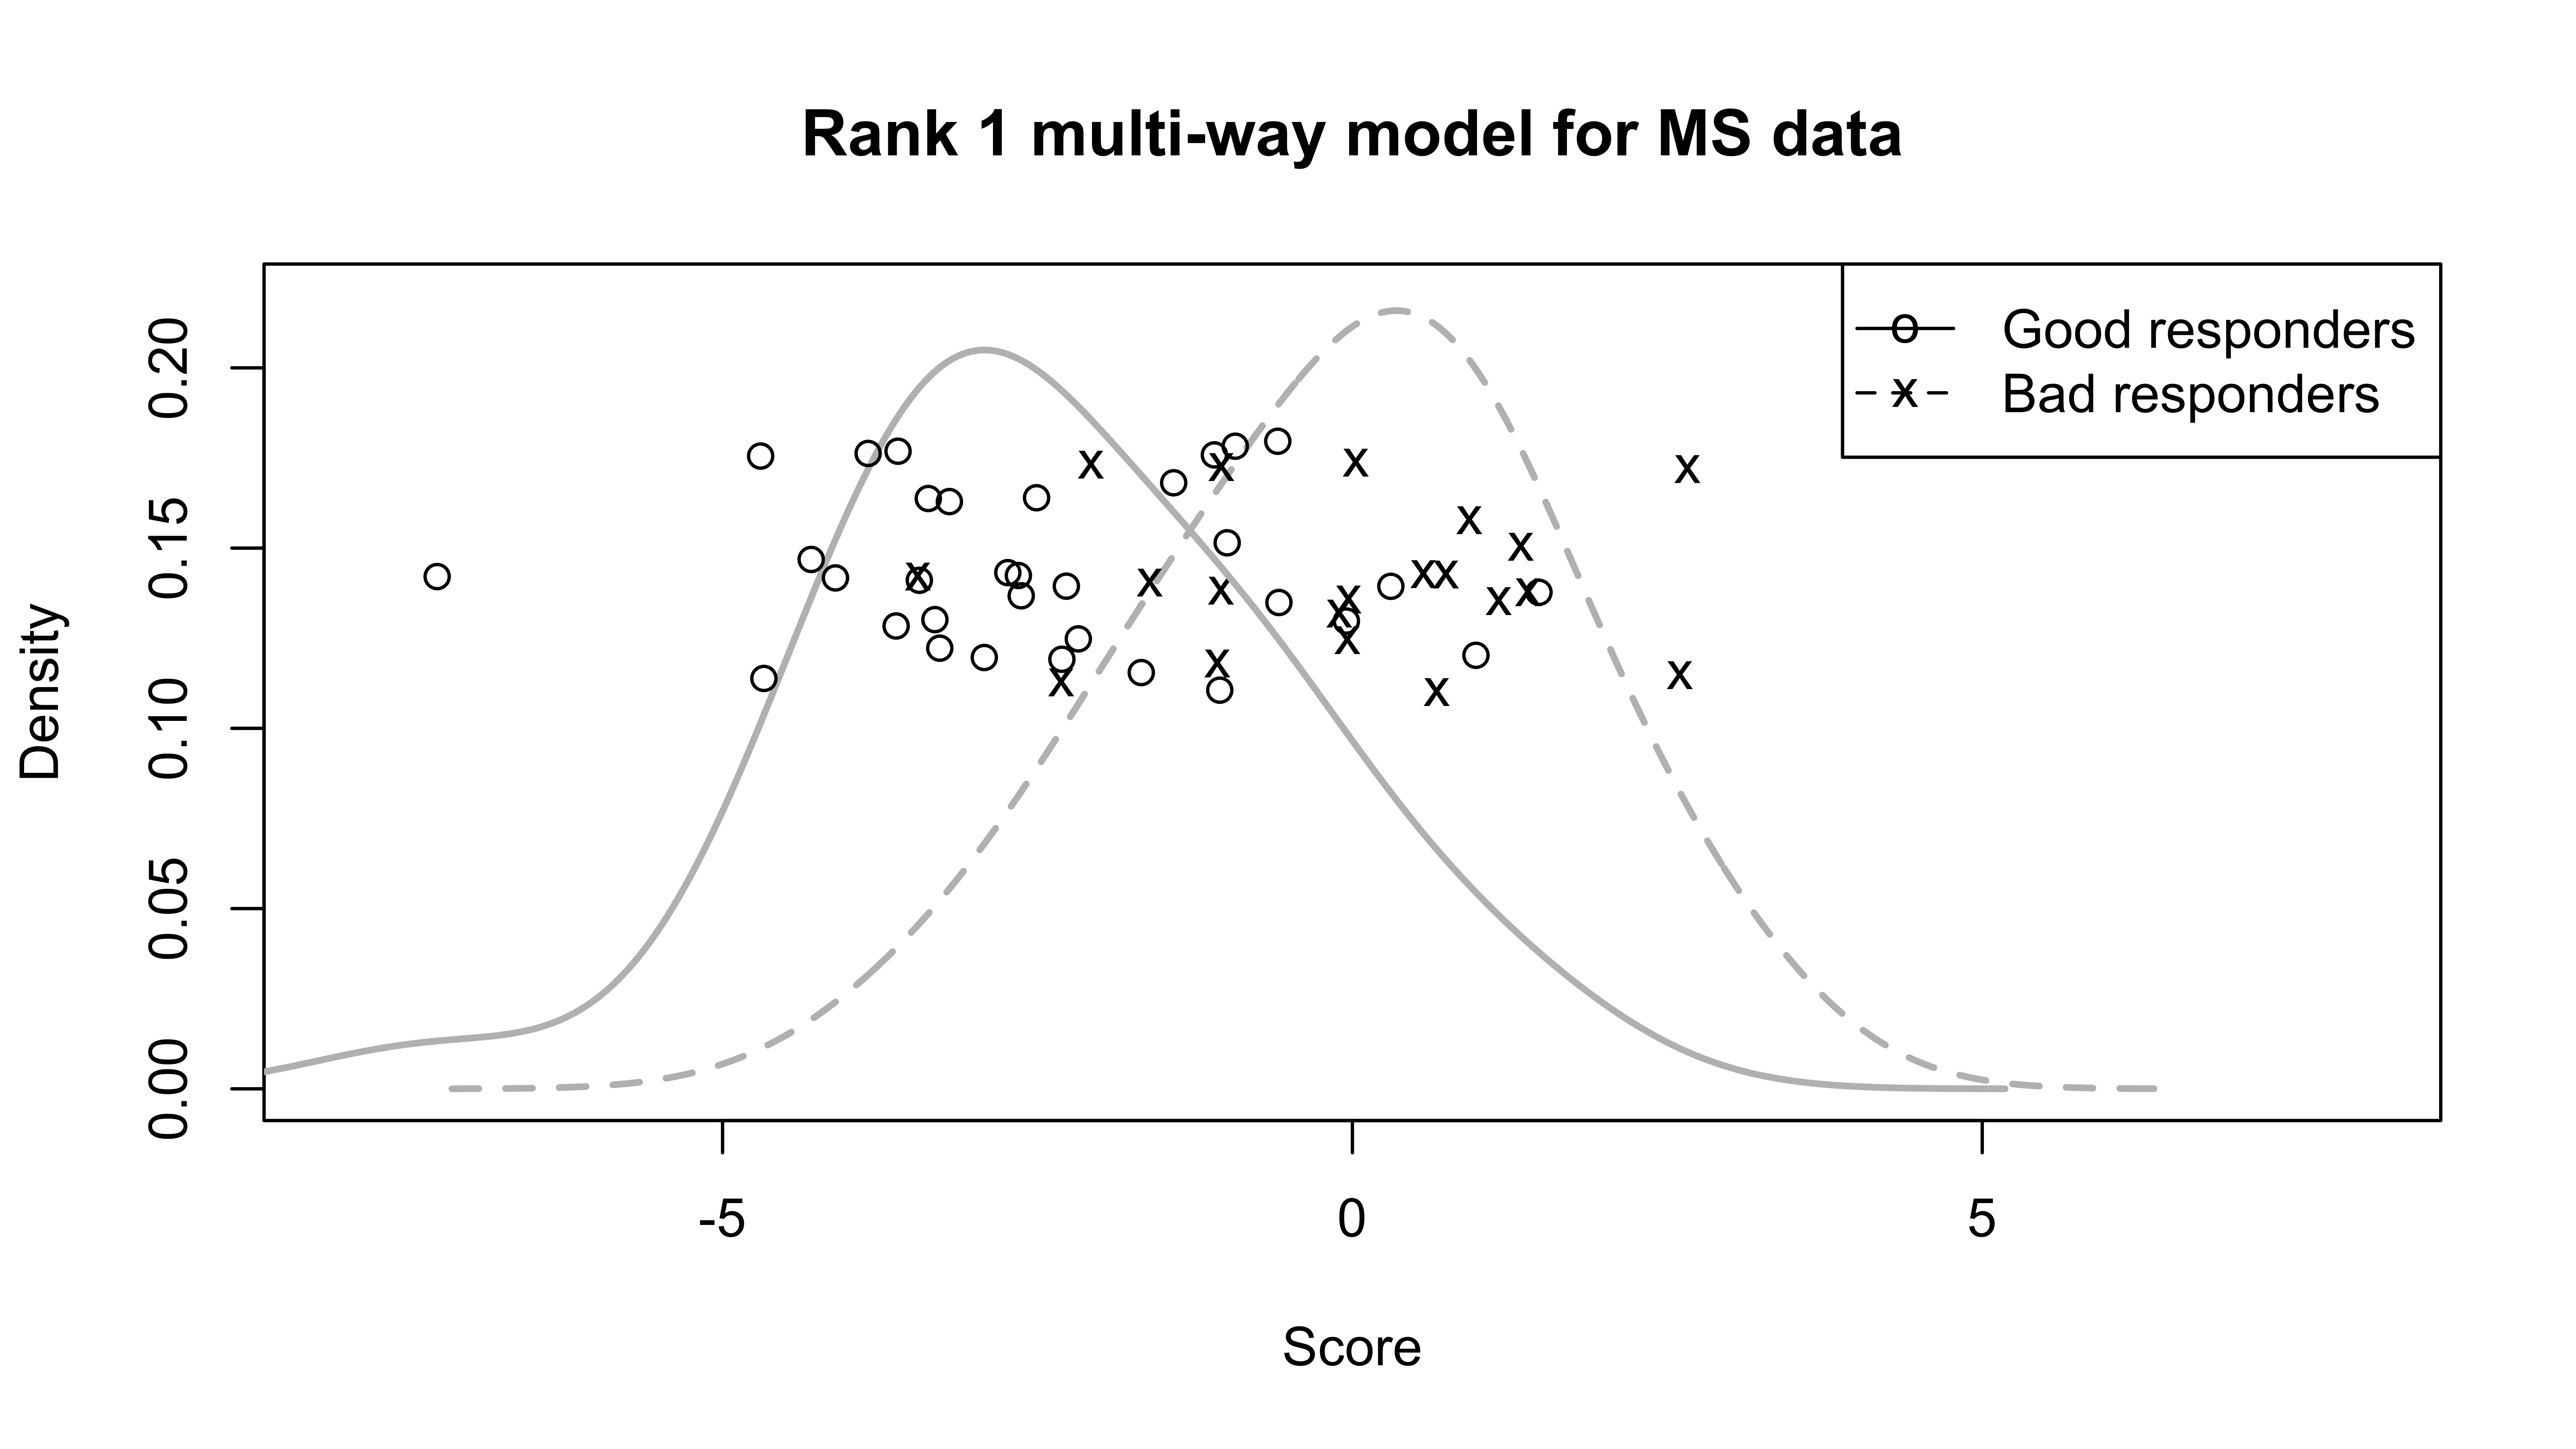
\includegraphics{TimeCourseScores_INFB.png}

\subsection{Coefficients and bootstrap confidence
intervals}\label{coefficients-and-bootstrap-confidence-intervals}

The rank 1 DWD coefficients are given by one set of weights
correspoinding to time (\texttt{results.mw\$w}) and one set of weights
corresponding to genes (\texttt{results.mw\$v}). We generate 5000
bootstrap samples to assess variability of these coefficients (this can
be computationally intensive, we recommend lowing the number of
bootstrap samples if necessary):

\begin{verbatim}
dwdvec.time.boot = matrix(nrow=7,ncol = 5000)
dwdvec.gene.boot = matrix(nrow=76,ncol = 5000)
for(i in 1:5000){
  samp1 = sample(c(1:53)[Class==1],20, replace=TRUE)
  samp2 = sample(c(1:53)[Class==2],33, replace=TRUE)
  index = c(samp1,samp2)
  results.boot <- mul.dwd(DataArray[index,,],y=as.factor(Class[index]), rank=1)
  dwdvec.time.boot[,i] <- results.boot[[2]]
  dwdvec.gene.boot[,i] <- results.boot[[3]]
}
\end{verbatim}

We then plot the coefficients, with 95\% bootstrap confidence intervals:

\begin{verbatim}
png(filename = "TimeCourseCoefficients_INFB.png",width=8,height=6,units='in',res=800)
plot1 <- ggplot(Summary, aes(x = GeneNames, y = GeneCoeffs)) +  
  labs(x="Genes",y = "Coefficients")+
  geom_bar(position = position_dodge(), stat="identity", fill="gray") + 
  geom_errorbar(aes(ymin=estimates.lower.gene, ymax=estimates.upper.gene), width=0.50) +
  ggtitle("DWD coefficients (genes)") + # plot title
  theme_bw() + # remove grey background 
  theme(panel.grid.major = element_blank(),axis.text.x=element_blank(),axis.ticks.x=element_blank()) +# r
  geom_hline(yintercept = 0)
plot2 <- ggplot(SumTime, aes(x = Time, y = Coeffs)) +  
  labs(x="Time",y = "Coefficients")+
  geom_bar(position = position_dodge(), stat="identity", fill="gray") + 
  geom_errorbar(aes(ymin=estimates.lower.time, ymax=estimates.upper.time), width=0.50) +
  ggtitle("DWD coefficients (time)") + # plot title
  theme_bw() + # remove grey background 
  theme(panel.grid.major = element_blank()) +# r
  geom_hline(yintercept = 0)
grid.arrange(plot1,plot2,nrow=2)
dev.off()
\end{verbatim}

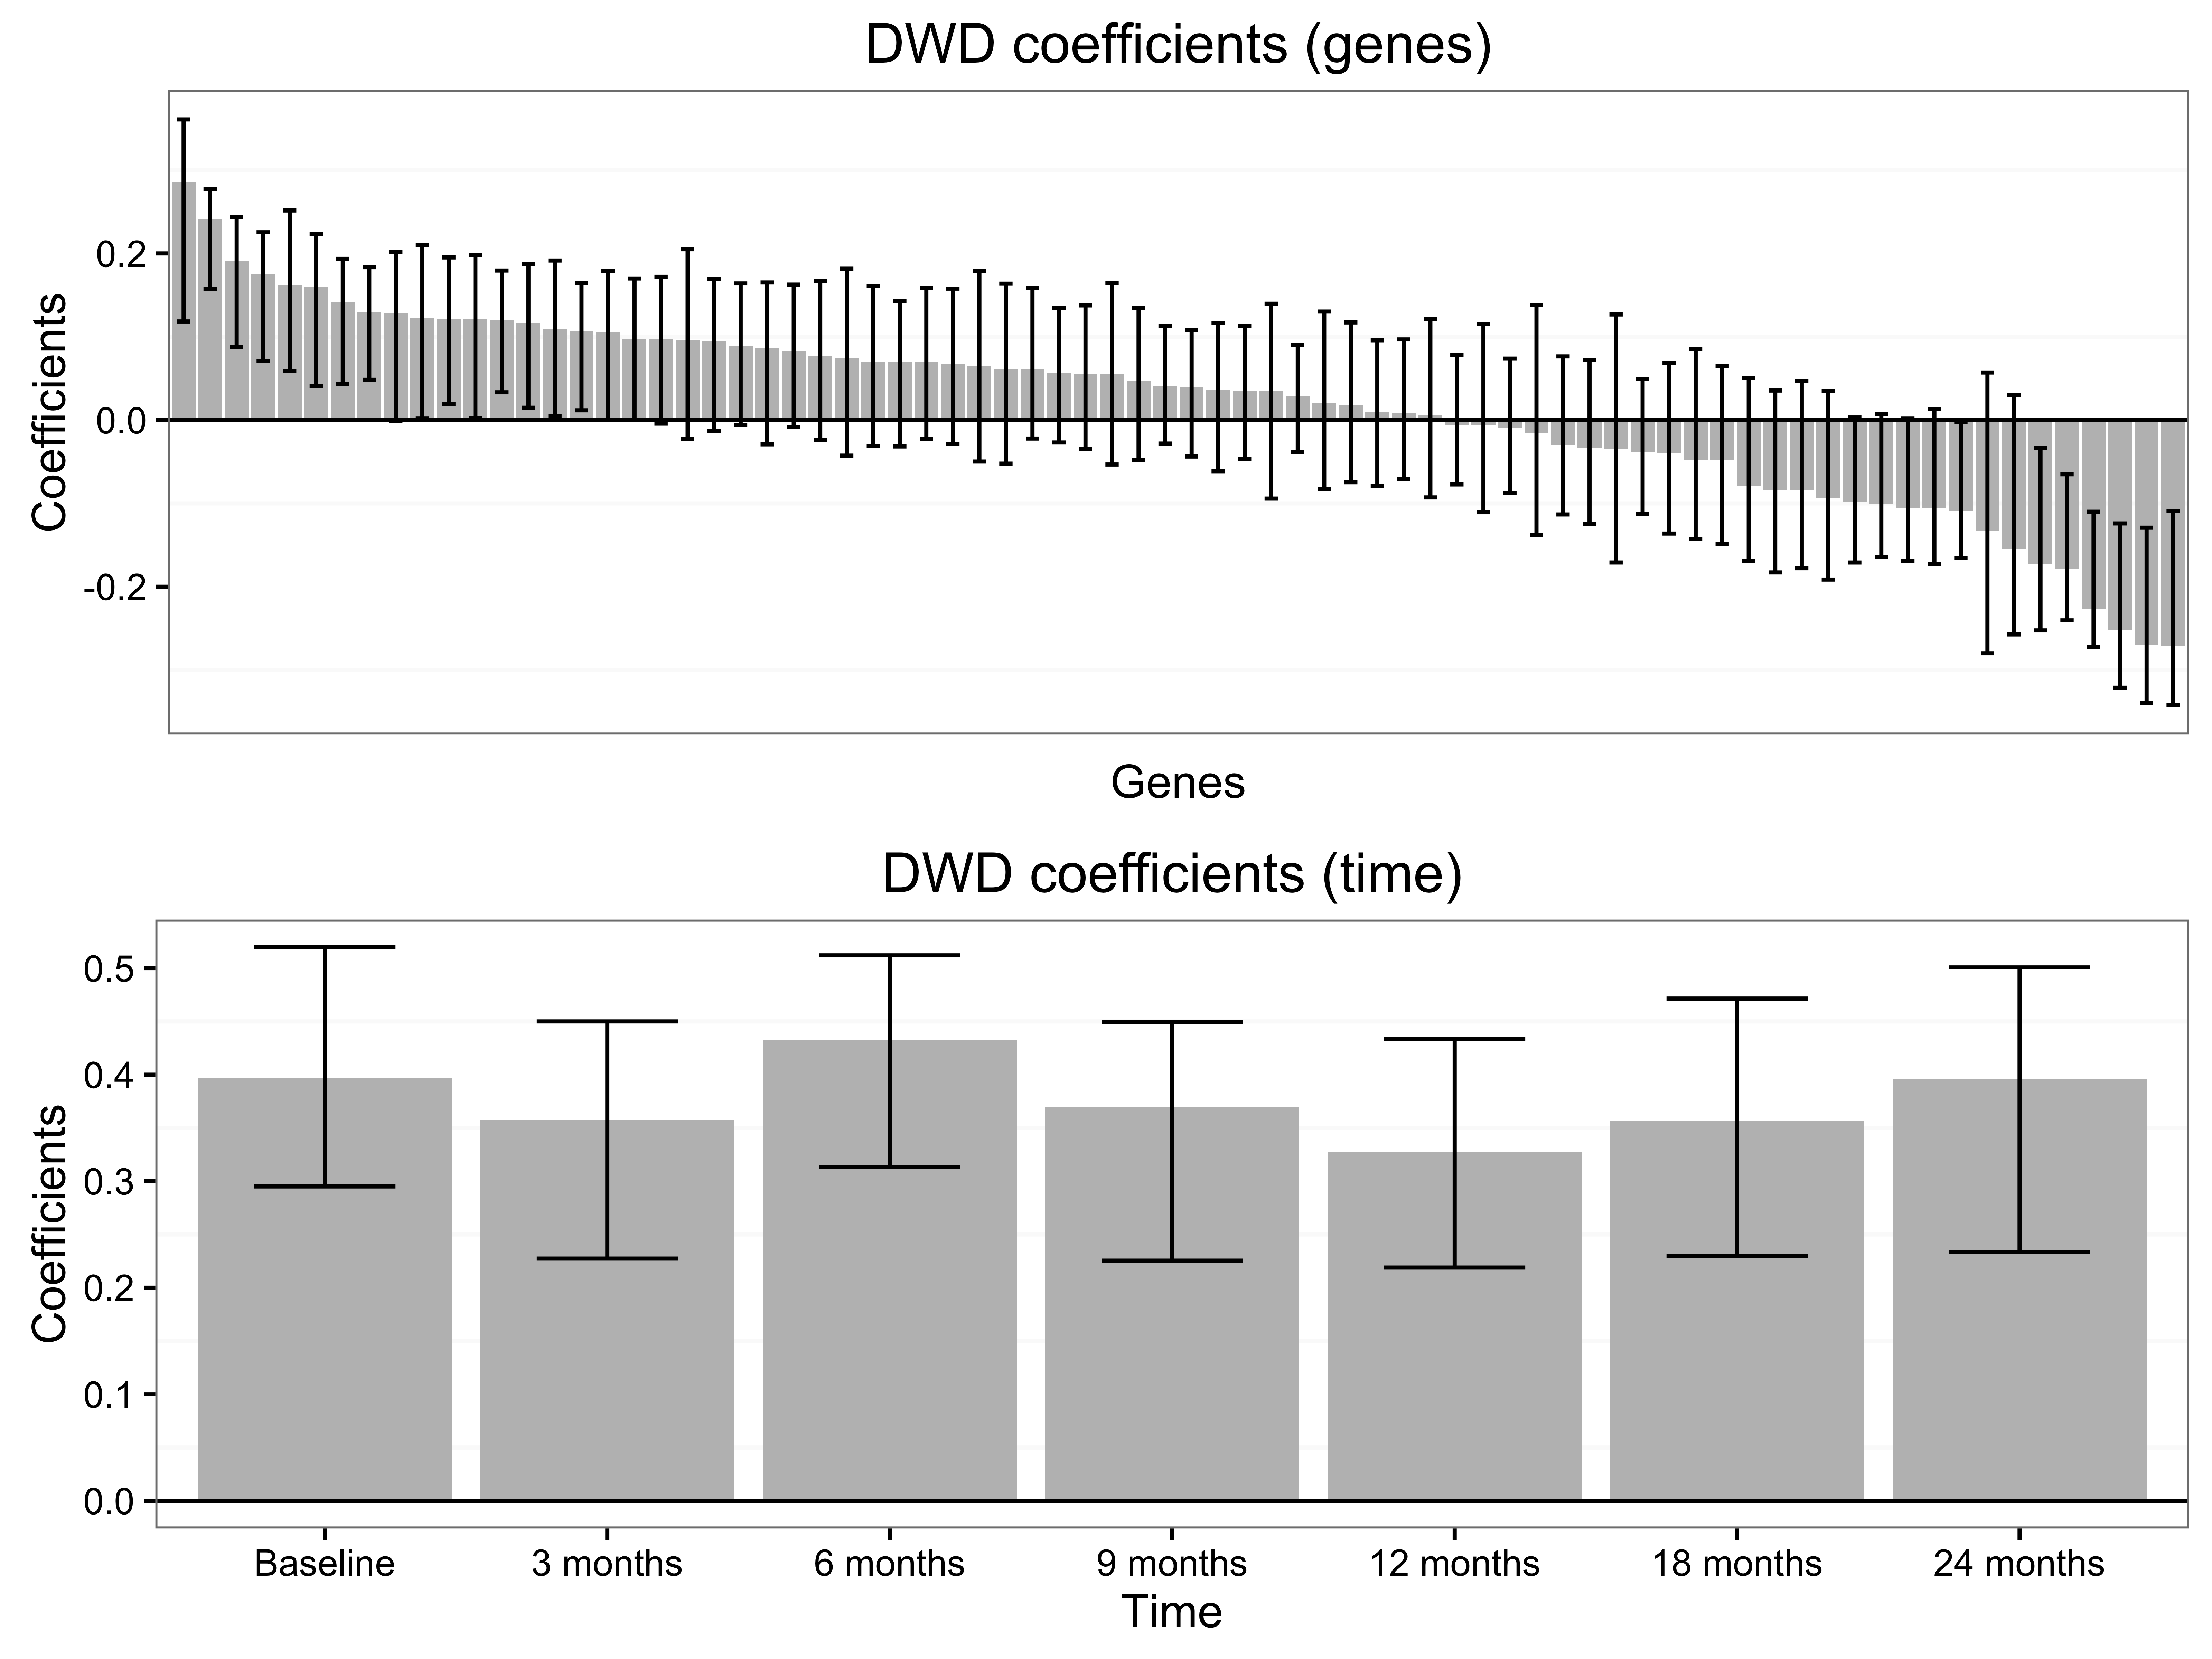
\includegraphics{TimeCourseCoefficients_INFB.png}

\subsection*{References}\label{references}
\addcontentsline{toc}{subsection}{References}

Baranzini, Sergio E, Parvin Mousavi, Jordi Rio, Stacy J Caillier, Althea
Stillman, Pablo Villoslada, Matthew M Wyatt, et al. 2005.
``Transcription-Based Prediction of Response to IFN$\beta$ Using
Supervised Computational Methods.'' \emph{PLoS Biol} 3 (1). Public
Library of Science: e2.

\end{document}
